A common paradigm in concurrent programming is that of \emph{interacting
  peers}.  Several threads or processes are peers, in the sense that they
execute basically the same code.  They exchange messages to achieve some goal.
The way in which messages are exchanged can follow various patterns or
topologies.

\begin{figure}[hbtp]
%\begin{center}
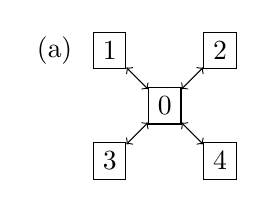
\begin{tikzpicture}[scale = 0.7]
\draw(-2,1) node {(a)};
\draw(0,0) node[draw] (0) {0};
\draw(-1,1) node[draw] (1) {1}; \draw[<->] (0) -- (1);
\draw(1,1) node[draw] (2) {2}; \draw[<->] (0) -- (2);
\draw(-1,-1) node[draw] (3) {3}; \draw[<->] (0) -- (3);
\draw(1,-1) node[draw] (4) {4}; \draw[<->] (0) -- (4);
\end{tikzpicture}
%%%%%
\hfil
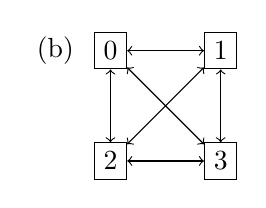
\begin{tikzpicture}[scale = 0.7]
\draw(-2,1) node {(b)};
\draw(-1,1) node[draw] (0) {0};
\draw(1,1) node[draw] (1) {1}; 
\draw(-1,-1) node[draw] (2) {2};
\draw(1,-1) node[draw] (3) {3}; 
\foreach \x in {1,...,3}  \draw[<->] (0) -- (\x);
\foreach \x in {2,...,3}  \draw[<->] (1) -- (\x);
\draw[<->] (2) -- (3);
\end{tikzpicture}
%%%%% Ring
\hfil
\def\r{1.4}
\raisebox{-1.9mm}{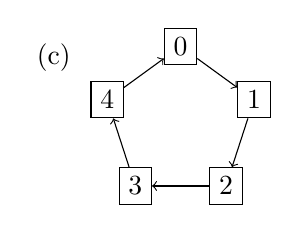
\begin{tikzpicture}[scale = 0.7]
\draw(-2.3,1.2) node {(c)};
\foreach \i in {0,...,4} 
  \draw (90-72*\i: \r) node[draw] (\i) {\i}; 
\foreach \i/\j in {0/1, 1/2, 2/3, 3/4, 4/0} \draw[->] (\i) -- (\j);
%% \draw(-1,1) node[draw] (0) {0};
%% \draw(1,1) node[draw] (1) {1}; 
%% \draw(-1,-1) node[draw] (3) {3};
%% \draw(1,-1) node[draw] (2) {2}; 
%% \draw[->] (0) -- (1); \draw[->] (1) -- (2); 
%% \draw[->] (2) -- (3); \draw[->] (3) -- (0);
\end{tikzpicture}}
%%%%% Heap
\hfil
\raisebox{-2.9mm}{
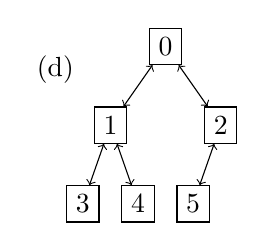
\begin{tikzpicture}[xscale = 0.7, yscale = 1.0]
\draw(-2,-0.3) node {(d)};
\draw(0,0) node[draw] (0) {0};
\draw (0)++(-1,-1) node[draw] (1) {1}; \draw[<->] (0) -- (1);
\draw (0)++(1,-1) node[draw] (2) {2}; \draw[<->] (0) -- (2);
\draw (1)++ (-0.5,-1) node[draw] (3) {3}; \draw[<->] (1) -- (3);
\draw (1)++ (0.5,-1) node[draw] (4) {4}; \draw[<->] (1) -- (4);
\draw (2)++ (-0.5,-1) node[draw] (5) {5}; \draw[<->] (2) -- (5);
% \draw (2)++ (0.5,-1) node[draw] (6) {6}; \draw[<->] (2) -- (6);
\end{tikzpicture}}%
%\end{center}
\caption{Four patterns of interacting peers: (a) a centralised pattern; (b)~a
  fully connected topology; (c) a ring; (d) a binary heap.}
\label{fig:interacting-peers}
\end{figure}

%%%%%

In this chapter we will examine four patterns of interacting peers, depicted
in Figure~\ref{fig:interacting-peers}: 
%
\begin{enumerate}
\item[(a)] A system with a centralised thread doing most of the work;

\item[(b)] A symmetric, fully connected topology, where each thread sends
  messages to all the others;

\item[(c)] A ring topology, where each thread communicates with just its two
  neighbours;

\item[(d)] A binary tree, or heap, topology, where each thread communicates
  just with its parent and two children.
\end{enumerate}
%
We will often use graph-theoretic terminology, and refer to the threads as
\emph{nodes}.  

Typically, each node will hold some data, and they want to calculate some
function of that data.  To illustrate different topologies and associated
techniques, we consider a very simple example in the first part of this
chapter: at the start, each node holds an integer; at the end, each node
should hold the sum of all those integers.
%
For each pattern, we will implement objects implementing the following trait. 
\begin{scala}
/** The trait specifying the various sum examples.
  * Each thread calls apply, passing in its value, and gets back the overall
  * sum. */
trait Sum{
  /** Submit value, and receive back overall sum. 
    * @param £me£ the identity of this thread.
    * @param £x£ the value submitted. */
  def apply(me: Int, x: Int): Int
}
\end{scala}

%%%%%

We will reason about the correctness of the patterns by identifying
\emph{invariants} that hold at certain points in the execution, for example,
about the values sent in particular messages, or properties of the state of
threads after each message that is sent or received.

We will also consider the cost of each pattern.  One obvious measure of cost
is the \emph{total} number of messages sent.  However, this isn't necessarily
a good measure of the running time if multiple messages can be sent
concurrently.
%
We will therefore also consider the number of messages sent
\emph{sequentially}.  Recall the ``happens-before'' relation $\preceq$; we say
that messages $m_1$, \ldots, $m_k$ form a \emph{totally ordered chain} if
necessarily 
\[\mstyle
m_1 \prec m_2 \prec \ldots \prec m_k,
\]
i.e., those messages have to be sent in that sequential order.  We will be
interested in identifying the length of the longest totally ordered chain, and
how that relates to the number of threads.

In the second half of this chapter, we consider two examples suitable for
distributed systems.  The first considers a ring topology, with the goal of
electing one of the nodes as a leader or controller.  The second example
considers a more general graph, where one node is designated as the
controller, each node knows only about its neighbours, and the goal is to find
all the nodes reachable from the controller, and to construct a spanning tree
for those nodes.


%%%%%%%%%%%%%%%%%%%%%%%%%%%%%%%%%%%%%%%%%%%%%%%%%%%%%%%%%%%%

\section{Centralised Pattern}

We start with the centralised pattern: see Figure~\ref{fig:sum-centralised}.
In this protocol, each client node sends its value to a central node, with
identity~|0|.  The controller calculates the sum, and sends the sum back.
We use a single channel in each direction, which is shared by the client
nodes.  This pattern has similarities with the client-server pattern we
studied in Chapter~\ref{chap:clientServer}, except the controller has its own
value. 

%%%%%

\begin{figure}[bht]
\begin{scala}
/** Implementation of £Sum£ using a controller.  The controller is the node
  * with identity £0£. */
class Centralised(n: Int) extends Sum{
  private val toController = new BuffChan[Int](n-1 max 1)
  private val fromController = new BuffChan[Int](n-1 max 1)

  def apply(me: Int, x: Int): Int = {
    if(me == 0){ // This is the controller.
      var sum = x
      // Receive values from other threads.
      for(i <- 1 until n){ val w = toController?(); sum += w }
      // Distribute sum.
      for(i <- 1 until n) fromController!sum
      sum
    }
    else{
      toController!x     // Submit my value.
      fromController?() // Get back the result.
    }
  }
}
\end{scala}
\caption{The sum example using the centralised pattern.}
\label{fig:sum-centralised}
\end{figure}

%%%%%

Arguing for the correctness of this program is straightforward.
Write $x_i$ for the value chosen by node~$i$.  Then during the first stage of
the protocol, the following invariant holds for the controller:
%
\begin{eqnarray*}
\sm{sum} & = & 
   x_0 + \sum \set{x_i \| 1 \le i < \sm n \land 
           \mbox{node~$i$'s value has been received}}.
\end{eqnarray*}
%
At the end of the |for| loop, the controller has received all the values, so
|sum| holds the desired result. 

\begin{instruction}
Make sure you understand the details of this program and the correctness
argument.
\end{instruction}

%%%%%

We can test the program, and the ones in subsequent sections, against
a sequential specification.  We arrange for each thread to pick a random value
for~|x|, write it into a global array~|xs| (indexed by thread identities, to
avoid race conditions), use the |Sum| object to obtain the purported sum, and
write it to a global array~|results| (again indexed by thread identities).  We
then calculate the correct sum sequentially (as |xs.sum|) and check that each
element of |results| is as expected.

%%%%%

This protocol uses $2(\sm n-1)$ messages in total: each client thread sends one
message and receives one message.  However, none of these messages can occur
concurrently, since all messages involve the controller.
Write $\sm{toController}.i$ for the communication on |toController| from
thread~$i$, and similarly for |fromController|.
We can find a totally-ordered chain of communications:
\[
\begin{align}
\mbox{\SCALA{toController}}.i_1 \prec \mbox{\SCALA{toController}}.i_2 
  \prec \ldots  \prec \mbox{\SCALA{toController}}.i_{\ss n-1} \prec \\
\qquad
  \mbox{\SCALA{fromController}}.j_1 \prec \mbox{\SCALA{fromController}}.j_2 
  \prec \ldots \mbox{\SCALA{fromController}}.j_{\ss n-1}
\end{align}
\]
for some permutations $i_1, \ldots, i_{\ss n-1}$ and $j_1, \ldots, j_{\ss
  n-1}$ of $1, \ldots, \sm n-1$.


%%%%%%%%%%%%%%%%%%%%%%%%%%%%%%%%%%%%%%%%%%%%%%%%%%%%%%%

\section{Fully Connected Pattern}

We now consider the fully connected pattern: see
Figure~\ref{fig:sum-symmetric}.  In this solution, each node sends its value
to every other node, and each node calculates the sum using the values it
receives.

%%%%%

\begin{figure}[htbp]
\begin{scala}
/** Implementation of £Sum£ using the symmetric (fully connected) pattern. */
class Symmetric(n: Int) extends Sum{
  /** Channels to send to nodes, indexed by the receivers' identities. */
  private val toNode = Array.fill(n)(new BuffChan[Int](n-1 max 1))

  def apply(me: Int, x: Int): Int = {
    for(i <- 0 until n) if(i != me) toNode(i)!x }
    // Receive values.
    var sum = x // Sum so far.
    for(i <- 1 until n){ val w = toNode(me)?(); sum += w }
    sum
  }
}
\end{scala}
\caption{The sum example using a fully connected topology.}
\label{fig:sum-symmetric}
\end{figure}

%%%%%

Each node needs to send $\sm{n}-1$ messages, and receive $\sm{n}-1$ messages.
We give each node its own channel on which it can receive messages.  We
arrange for the two stages to be performed sequentially.  However, in order to
avoid deadlocks, we need to make the channels buffered with capacity (at
least) |n-1|, so all the threads can send before any is ready to receive (when
$\sm n = 1$, we give the channels capacity~$1$, because the capacity fo a
|BuffChan| must be strictly positive).  Alternatively, we could have run the
two stages concurrently, using a separate thread for each, in which case we
could have used synchronous channels.

Write $x_j$ for the value chosen by node~$j$.  Then during the receiving loop,
each node~$i$ has a value for \SCALA{sum} such that:
%
\begin{eqnarray*}
\sm{sum} & = & 
  x_i + \sum \set{x_j \| \mbox{node~$j$'s value has been received by node~$i$}}.
\end{eqnarray*}
%
Each node sends to each other node; and each node receives exactly $\sm n-1$
times; hence each node must receive each other node's value.  This means that
each node's final value for |sum| is the correct sum.

\begin{instruction}
Make sure you understand the details of the code and the correctness
argument.
\end{instruction}

%%%%%

The above program suffers from contention.  
Each \SCALA{sender} sends to the other nodes in order, starting from
\SCALA{0}.  This means that:
%
\begin{itemize}
\item
Initially, all the nodes are contending to send to node~\SCALA{0}, so most
will be temporarily blocked;

\item
Node $\sm n-1$ has to wait until another node has finished sending to
\emph{all} other nodes before receiving \emph{anything}.  %% This gives a chain
%% of length $2\sm{n}-3$ ($\sm n-2$ sends before this node receives anything,
%% and then $\sm n-1$ receives by this node).
\end{itemize}

A better approach is for each node to send in a different order, say starting
from the one with identity one higher than itself:
%
\begin{scala}
  for(i <- 1 until n) toNode((me+i)%n)!x 
\end{scala}
%
If all the nodes proceed at the same speed, this is likely to avoid contention
for the channels.  Of course, unfortunately scheduling might create
contention; but this seems unlikely. 

%%%%%

This protocol uses $\sm n(\sm n-1)$ messages in total, with sequential chains
of length~$2(\sm n -1)$.  The $O(\sm n^2)$ total number of messages means that
a fully connected topology has rather a large communication overhead: each of
the other patterns uses fewer messages. 
